\chapter{�bersicht}

	\section{Was ist Steganographie}
	
	Die Steganographie ist eine Methode die sich mit dem verstecken von zu �bermittelnden Nachrichten besch�ftigt und kam schon in der Antike zum Einsatz. Das Wort kommt aus den griechischen W�rter ''stegano'' und ''graphein'', was �bersetzt ''bedeckt schreiben'' bedeutet \cite{L: StegoGeschichte}. Dabei wird meist ein Text, aber auch andere Arten von Informationen, in einem Tr�germedium versteckt. Diese Kombination wird als Steganogramm bezeichnet. Das Medium sollte so gew�hlt sein, das sich die einzubettenden Daten leicht integrieren lassen. Au�erdem ben�tigt es ein gewisses Ma� an Entropie damit Unregelm��igkeiten nicht so stark auffallen, denn eine Blume ist in einer bunten Blumenwiese schwerer zu finden als auf einem asphaltierten Parkplatz. Ziel ist es immer, die Wahrnehmungsschwelle eines Menschen so zu unterschreiten, dass niemand auf die Idee kommt �berhaupt nach einer versteckten Nachricht zu suchen. 
	\todo{Welche Techniken wof�r gut sind und welche Tr�germaterialen man braucht wird in den sp�teren abschnitten behandelt}
	
	
	Die M�glichkeiten f�r Steganogramme haben sich mit der Entwicklung von Computer und elektronischer Datenverarbeitung sehr stark ver�ndert, die Idee dahinter ist jedoch die gleiche: Wir verstecken Informationen.
	Fr�her hat man noch Beispielsweise mit Unsichtbarer Tinte geschrieben, welche erst mit Hitze sichtbar wird (\zb Zitronensaft). Auch wurden Techniken wie etwa die monoalphabetische Substituion benutzt, bei welcher Buchstaben des zu versteckenden Wortes �ber eine Tabelle durch W�rter ersetzt werden. Diese Wortfolge wird dann mit weiteren nicht in der Tabelle vorkommenden Worten erg�nzt um vollst�ndige, grammatikalisch korrekte S�tze bilden zu k�nnen. Eine solche Tabelle findet man zum Beispiel in dem Buch 1 der Polygraphia von Johannes Trithemius (Siehe: \autoref{fig:L: Polygraphia}).
	
	\begin{figure}[H]
		\centering
		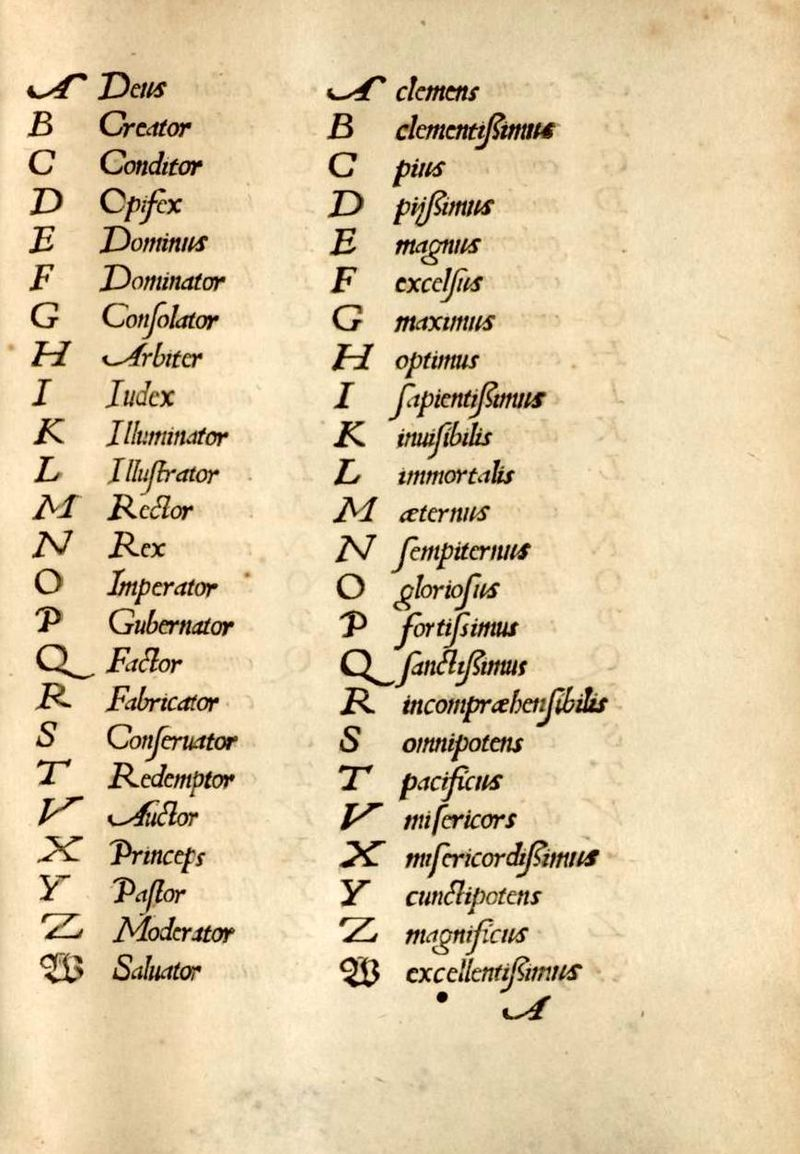
\includegraphics[scale=1.1]{images/L-Trithemius-Polygraphiae-71.jpg}
		\caption{Buchstaben-Wort-Substitutionstabelle von Buch I der Polygraphia von Johannes Trithemius, Quelle: \url{http://daten.digitale-sammlungen.de/bsb00026190/image_71}}
		\label{fig:L: Polygraphia}
	\end{figure}
	
	
	
	
	
	
	\section{Einsatzgebiete}
	
	
	
	\section{Vor- und Nachteile}
	
	\section{Abgrenzung zur Kryptographie}
	
	Kryptographie und Steganographie werden oft gemeinsam verwendet, wodurch meist nicht genau zwischen diesen beiden Verfahren unterschieden wird. Wie man in \autoref{L: Tab: Stego VS Crypto} \todo{Wie bekommt man die richtige Bezeichnung hier in den Text(unterschied zwischen label und caption)} sehen kann, wirken beide Techniken auf den ersten Blick sehr �hnlich, sind aber bei genauerer Betrachtung zwei komplett unterschiedliche Verfahren. Wichtig ist hier vor allem zu beachten: Steganographie sch�tzt Daten nicht vor Dritten, wenn diese gezielt danach Suchen und sich sicher sind, das in den Informationen die Ihnen vorliegen weitere Nachrichten versteckt wurden. Des weiteren haben Steganogramme die Eigenschaft zwar von Menschen schlecht erkannt werden zu k�nnen, von Computern jedoch meist relativ schnell durch Analysen und Vergleiche eine versteckte Nachricht sichtbar gemacht werden kann. \todo{Dazu mehr in den Punkten XYZ (z.B:) Wicked Problem} Dabei kommt es wieder sehr stark auf die verwendete Technik an. 
	
	Am Sichersten ist es wenn man beide Verfahren kombiniert. Dadurch hat man nicht nur die Vorteile der Kryptographie (Vertraulichkeit, Integrit�t und Authentizit�t), sondern auch die der Steganographie. Interessant ist hier vor allem die Eigenschaft von Verschl�sselungen: Diese gelten dann als sicher, wenn sie den Klartext derart ver�ndern, das er keine statistischen Merkmale des urspr�nglichen Text mehr aufweist. 
	Der Geheimtext ist dann nicht mehr von Rauschen zu unterscheiden. Wenn man dieses ''Rauschen'' dann mit Hilfe von Steganographie in ein unauff�lliges Tr�germedium einbettet, ist es selbst mit elektronischer Datenverarbeitung nicht mehr m�glich, eine Nachricht im Steganogramm zu entdecken. Die einzige M�glichkeit f�r Dritte hier noch etwas herauszufinden, ist das Steganogramm mit dem originalen Tr�germaterial zu vergleichen, hier fallen dann Unterschiede auf. Das ist aber selten machbar, denn die originalen Tr�germaterialien werden gleich nach der Erzeugung des Steganogramm nicht mehr gebraucht und k�nnen vernichtet werden.
	
	
	
	
	
	
	\begin{table}[h]
		\begin{center}
			\begin{tabular}{|l|l|}
				\hline
				\textbf{Steganographie} & \textbf{Kryptographie}\\
				\hline
				\hline
				stegano = verdeckt 	& krypte = geheim \\
				graphein = scrheiben & graphein = schreiben \\
				\hline
				Die Nachricht wird verborgen, & Die Nachricht wird verschl�sselt \\
				nicht verschl�sselt & nicht verborgen \\
				\hline
				Scheinbar existiert gar & Die Nachricht existiert, kann aber\\
				keine Nachricht & nicht gelesen werden \\
				\hline
				
			\end{tabular}
		\end{center}
		\caption{Vergleich zwischen Steganographie und Kryptographie, Quelle: \cite{L: Stego VS Crypto}} 
		\label{L: Tab: Stego VS Crypto}
	\end{table}
	
	
	
	
	\section{Steganographie als ''Wicked Problem''}